%% LyX 2.3.3 created this file.  For more info, see http://www.lyx.org/.
%% Do not edit unless you really know what you are doing.
\documentclass[english]{article}
\usepackage[T1]{fontenc}
\usepackage{float}
\usepackage{amsmath}
\usepackage{graphicx}
\usepackage{hyperref}
\usepackage{subcaption}

\makeatletter

\hypersetup{
    colorlinks=true,
    linkcolor=blue,
    filecolor=magenta,      
    urlcolor=cyan,
}
\urlstyle{same}

%%%%%%%%%%%%%%%%%%%%%%%%%%%%%% LyX specific LaTeX commands.
%% Because html converters don't know tabularnewline
\providecommand{\tabularnewline}{\\}

\makeatother

\usepackage{babel}
\begin{document}
\title{Project 2}
\author{Zachary Taylor,John Dinofrio, Cristian Bueno}
\maketitle

\part*{Problem 1}

\textbf{Here, we aim to improve the quality of the video sequence provided above. This is a video recording of a highway during night. Most of the Computer Vision pipelines for lane detection or other self-driving tasks require good lighting conditions and color information for detecting good features. A lot of pre-processing is required in such scenarios where lighting conditions are poor. Now, using the techniques taught in class your aim is to enhance the contrast and improve the visual appearance of the video sequence. You can use any in-built functions for the same.}
\bigskip

The provided source video was extremely dark. We resize the image to both speed up our adjustments and make it easier to see the changes side by side with the image source.

\begin{figure}[H]
	\centering
		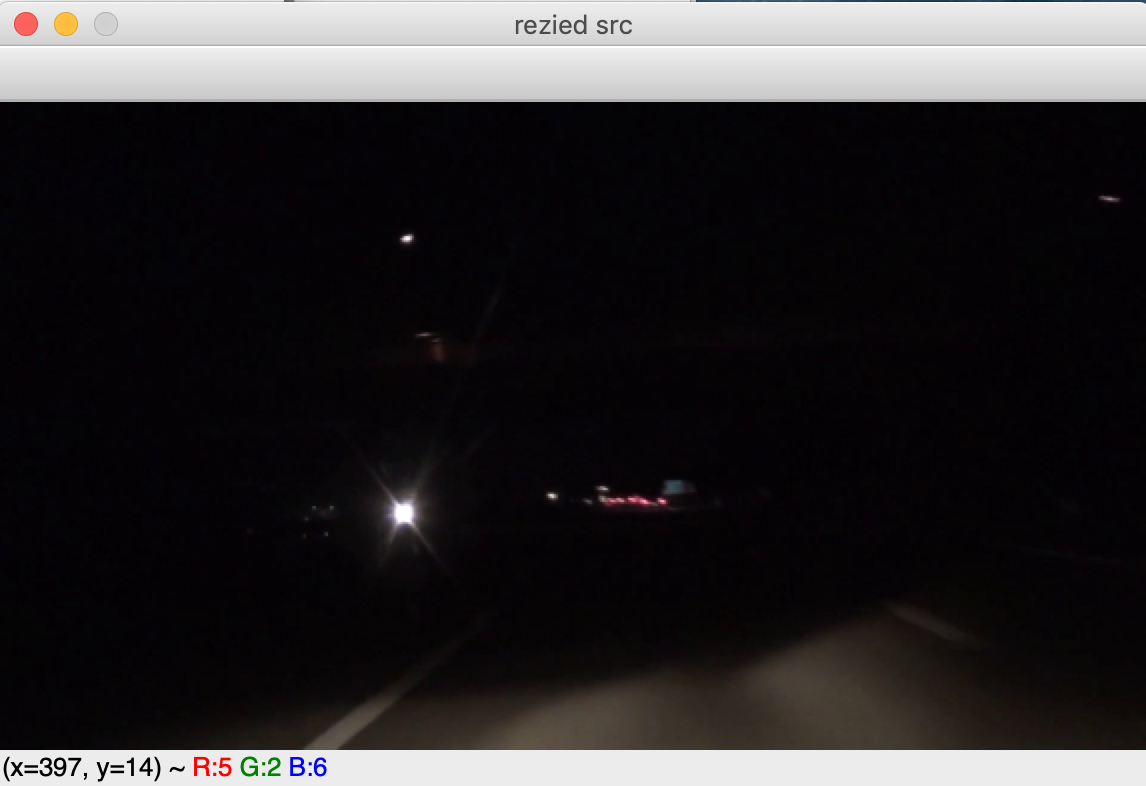
\includegraphics[width = 4in]{./images/src.png}
		\caption{Source Image}
\end{figure}

The first approach we took to solve this problem was using the histogram equalization technique as the effect as demonstrated in the course materials looked powerful. We utilized the built in OpenCV function called equalizeHist() to do this operation. Initially we made each frame grayscale and then equalized, but we also separated the three color channels, equalized each individually, and merged them back together into one image to try to get an equalized color image. We also tried other techniques of converting the image into other color spaces and trying to equalize certain channels that might increase the brightness and contrast, all with little improvement over the other methods. 

\begin{figure}[H]
	\begin{center}
		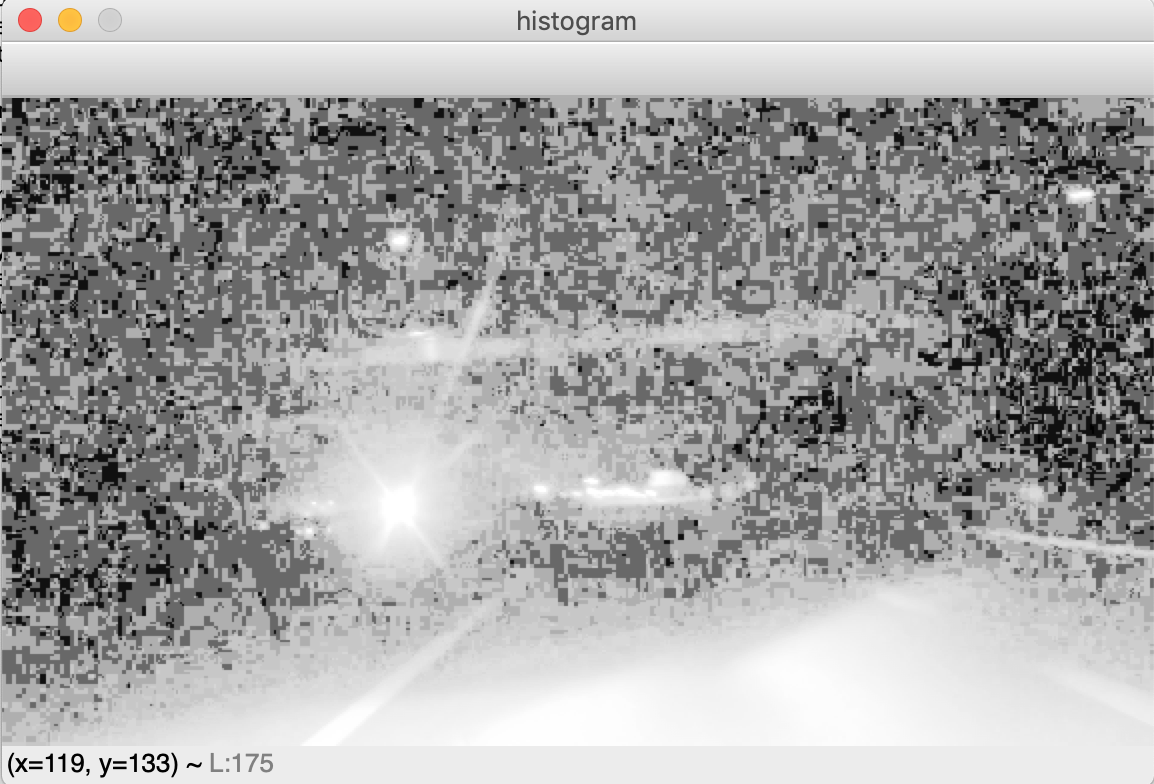
\includegraphics[width = 4in]{./images/gray.png}
	\end{center}
		\caption{Grayscale Histogram Equalization}
\end{figure}
\begin{figure}[H]
	\begin{center}
		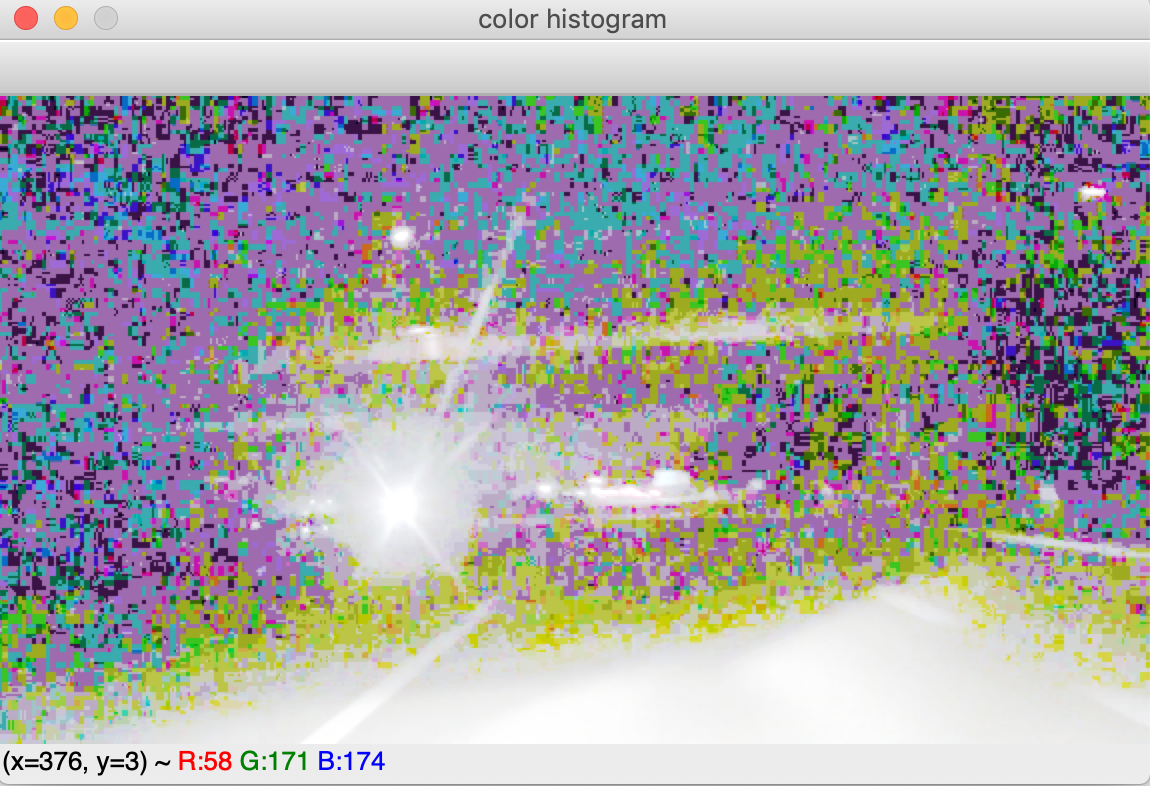
\includegraphics[width = 4in]{./images/color.png}
	\end{center}
		\caption{3 Channel Color Histogram Equalization}
\end{figure}
\begin{figure}[H]
	\begin{center}
		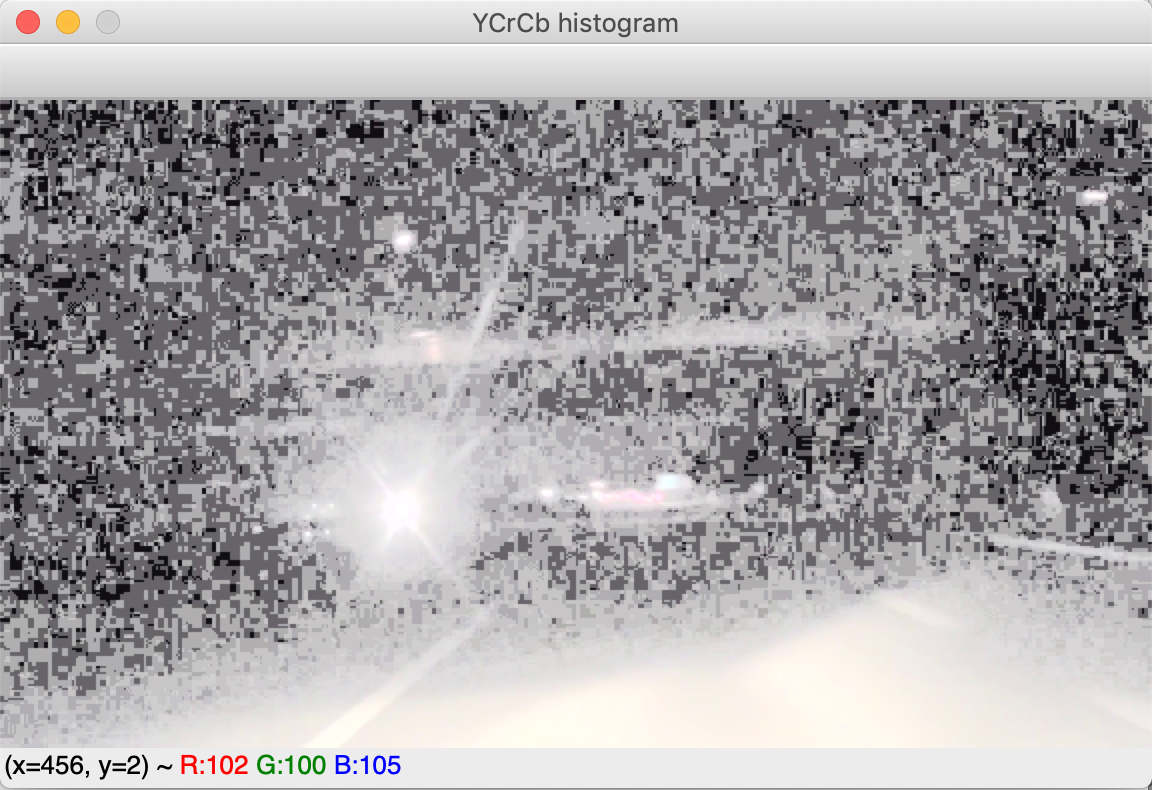
\includegraphics[width = 4in]{./images/yCrCb.png}
	\end{center}
		\caption{YCrCb Histogram Equalization}
\end{figure}

The consistent challenge we had using the built in histogram equalization is that we were getting a lot of noise in the image after equalizing. While it did make it slightly easier to see the lines on the road, the amount of noise in the image may make programmatically finding the lines on the road difficult. We were expecting results similar to what was shown in the class slides that brightened the image and exposed details that otherwise couldn't be seen, but instead got an image with so much noise it was hard to see anything in it. In analyzing the first frame of the video as a sample, we found that the first 25 intensity values on the grayscale image made up 90\% of the pixels in the image. Of those, there were 5 that represented 70\% of the image. Since such a large portion of the image was concentrated in such a narrow range, we can expect some pixelation to occur. This is specifically because each pixel value can only map to one new value, or in other words, we can't add more fidelity to the image than what is already there. That means, since 70\% of our image is populated by only 5 unique values, 70\% of our image, after equalization, will be made up of only 5 different intensity values, just further distributed across the full 8 bit intensity range. This result can be seen clearly by looking at the source and equalized histograms of the image below. Because these values are so spread out, the image looks pixelated instead of smooth. We can do some smoothing after the fact but then some detail is lost in the lane markings we are trying to uncover.

\begin{figure}[H]
	\begin{center}
		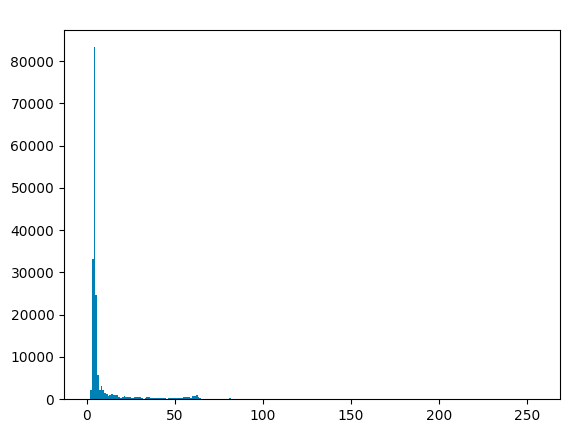
\includegraphics[width = 4in]{./images/grayHist.png}
	\end{center}
		\caption{Source Grayscale Histogram}
\end{figure}
\begin{figure}[H]
	\begin{center}
		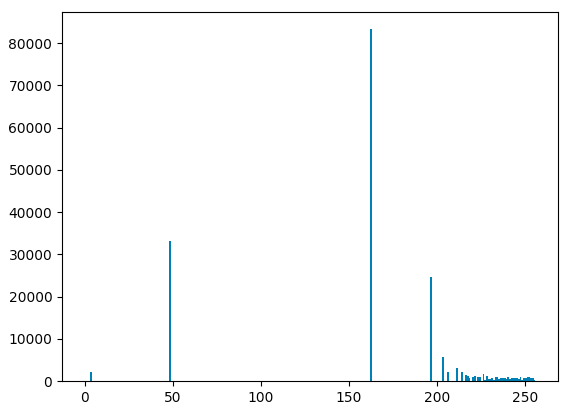
\includegraphics[width = 4in]{./images/grayEqualizedHist.png}
	\end{center}
		\caption{Equalized Histogram}
\end{figure}

Through some research and a desire to do better than what we got with the histogram equalization we were able to find another technique described that adjusts the "gamma" of the image. We found this method ultimately provided the best result of the methods we tested. Instead of trying to equalize the histogram, it maintains the same histogram shape but slides it to the right (increases) on the intensity value. Values starting with a lower intensity slide further to the right than those starting with a higher intensity value, which was also useful in this use case as we didn't want to over expose the light areas like the roads as it could ultimately wash out the lines as well. In effect, this increased the brightness of the overall image but maintains much of the same level of contrast from the source image. We were also able to maintain color correctness using this method as every color channel was adjusted at the same proportion, unlike when we equalized each color channel individually and merged them back together.
\begin{figure}[H]
	\begin{center}
		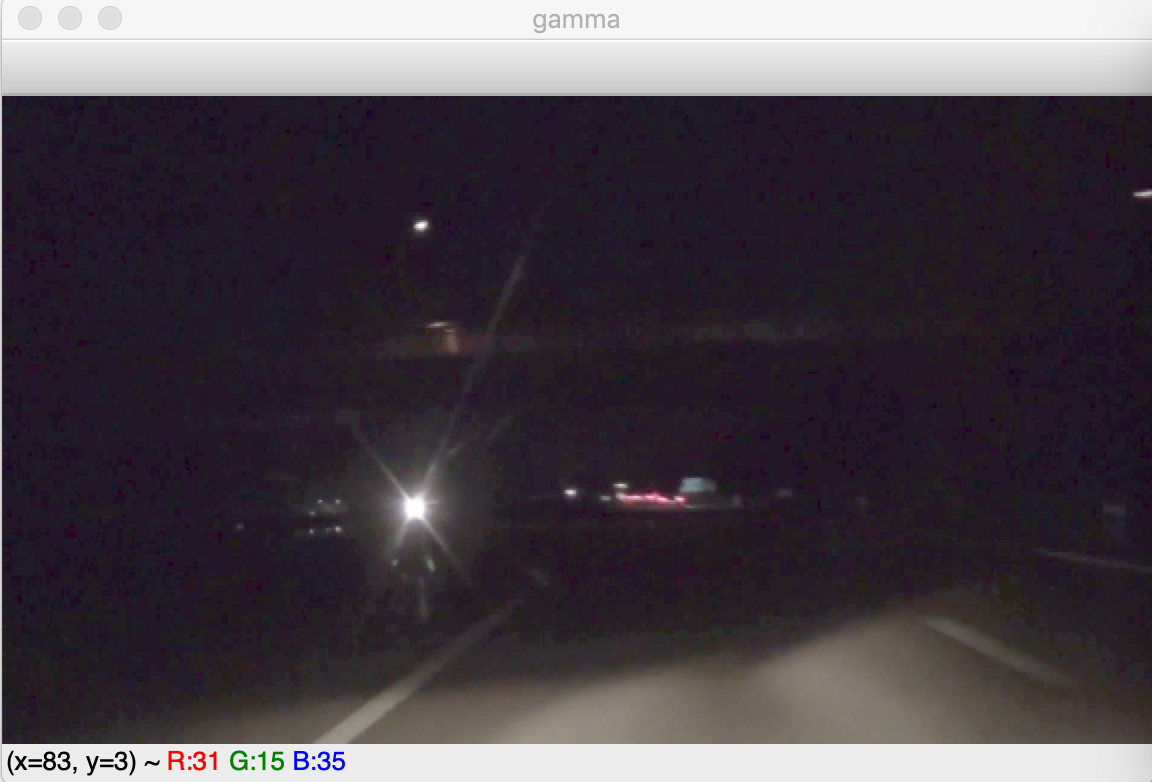
\includegraphics[width = 4in]{./images/gamma.png}
	\end{center}
		\caption{Gamma Adjustment}
\end{figure}
\begin{figure}[H]
	\begin{center}
		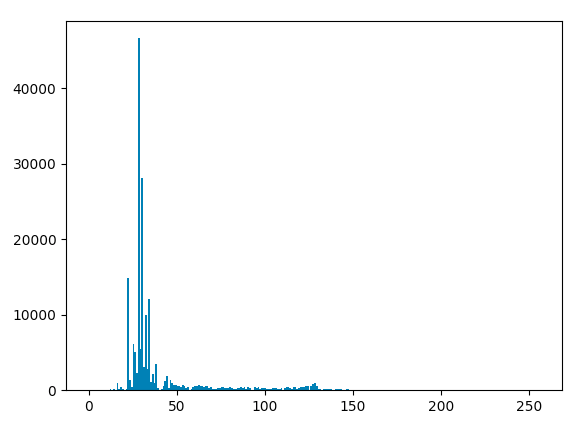
\includegraphics[width = 4in]{./images/gammaHist.png}
	\end{center}
		\caption{Gamma Adjustment Histogram}
\end{figure}

We recorded a video demonstrating the histogram equalization and the gamma adjustment techniques for the entire video sequence: \url{https://youtu.be/58KqZ3_qsso}
\part*{Problem 2}
\textbf{In this project we aim to do simple Lane Detection to mimic Lane Departure Warning systems used in Self Driving Cars. You are provided with two video sequences (both are required for this assignment), taken from a self driving car (click here to download). Your task will be to design an algorithm to detect lanes on the road, as well as estimate the road curvature to predict car turns.}
\end{document}
